\documentclass[a4paper,12pt]{article}

\usepackage[utf8x]{inputenc}
\usepackage[english, russian]{babel}

\usepackage{tabularx}
\usepackage{multirow}
\usepackage{graphicx}
\usepackage{misccorr}
\usepackage{indentfirst}


\usepackage{listings}
\usepackage{xcolor}

\usepackage{fullpage}

\usepackage[labelsep=endash,
		    margin=10pt, 
		    justification = centerlast, 
		    format = hang,
		    singlelinecheck=false
		    ]{caption}

\exhyphenpenalty=10000
\doublehyphendemerits=10000
\finalhyphendemerits=5000

\definecolor{codegreen}{rgb}{0,0.6,0}
\definecolor{codegray}{rgb}{0.5,0.5,0.5}
\definecolor{codepurple}{rgb}{0.58,0,0.82}
\definecolor{backcolour}{rgb}{0.95,0.95,0.92}
 
\lstdefinestyle{mystyle}{
    backgroundcolor=\color{backcolour},
    commentstyle=\color{codegreen},
    keywordstyle=\color{blue},
    numberstyle=\tiny\color{codegray},
    stringstyle=\color{codepurple},
    basicstyle=\footnotesize,
    breakatwhitespace=false,
    breaklines=true,
    captionpos=t,
    keepspaces=true,
    numbers=left,
    numbersep=5pt,
    showspaces=false,
    showstringspaces=false
    showtabs=false,
    tabsize=4,
    frame=tb
}
 
\lstset{style=mystyle}

\usepackage{color}
\usepackage{xcolor}
\usepackage{listings}
 
% Цвета для кода
 
\definecolor{string}{HTML}{B40000} % цвет строк в коде
\definecolor{comment}{HTML}{008000} % цвет комментариев в коде
\definecolor{keyword}{HTML}{1A00FF} % цвет ключевых слов в коде
\definecolor{morecomment}{HTML}{8000FF} % цвет include и других элементов в коде
\definecolor{сaptiontext}{HTML}{FFFFFF} % цвет текста заголовка в коде
\definecolor{сaptionbk}{HTML}{999999} % цвет фона заголовка в коде
\definecolor{bk}{HTML}{FFFFFF} % цвет фона в коде
\definecolor{frame}{HTML}{999999} % цвет рамки в коде
\definecolor{brackets}{HTML}{B40000} % цвет скобок в коде
 

%%% Отображение кода %%%
 
% Настройки отображения кода
 
\lstset{
	%morekeywords={*,...}, % если хотите добавить ключевые слова, то добавляйте	 
	% Настройки отображения     
	breaklines=true, % Перенос длинных строк
	% Для отображения русского языка
	extendedchars=true,
	literate={Ö}{{\"O}}1
	{Ä}{{\"A}}1
	{Ü}{{\"U}}1
	{ß}{{\ss}}1
	{ü}{{\"u}}1
	{ä}{{\"a}}1
	{ö}{{\"o}}1
	{~}{{\textasciitilde}}1
	{а}{{\selectfont\char224}}1
	{б}{{\selectfont\char225}}1
	{в}{{\selectfont\char226}}1
	{г}{{\selectfont\char227}}1
	{д}{{\selectfont\char228}}1
	{е}{{\selectfont\char229}}1
	{ё}{{\"e}}1
	{ж}{{\selectfont\char230}}1
	{з}{{\selectfont\char231}}1
	{и}{{\selectfont\char232}}1
	{й}{{\selectfont\char233}}1
	{к}{{\selectfont\char234}}1
	{л}{{\selectfont\char235}}1
	{м}{{\selectfont\char236}}1
	{н}{{\selectfont\char237}}1
	{о}{{\selectfont\char238}}1
	{п}{{\selectfont\char239}}1
	{р}{{\selectfont\char240}}1
	{с}{{\selectfont\char241}}1
	{т}{{\selectfont\char242}}1
	{у}{{\selectfont\char243}}1
	{ф}{{\selectfont\char244}}1
	{х}{{\selectfont\char245}}1
	{ц}{{\selectfont\char246}}1
	{ч}{{\selectfont\char247}}1
	{ш}{{\selectfont\char248}}1
	{щ}{{\selectfont\char249}}1
	{ъ}{{\selectfont\char250}}1
	{ы}{{\selectfont\char251}}1
	{ь}{{\selectfont\char252}}1
	{э}{{\selectfont\char253}}1
	{ю}{{\selectfont\char254}}1
	{я}{{\selectfont\char255}}1
	{А}{{\selectfont\char192}}1
	{Б}{{\selectfont\char193}}1
	{В}{{\selectfont\char194}}1
	{Г}{{\selectfont\char195}}1
	{Д}{{\selectfont\char196}}1
	{Е}{{\selectfont\char197}}1
	{Ё}{{\"E}}1
	{Ж}{{\selectfont\char198}}1
	{З}{{\selectfont\char199}}1
	{И}{{\selectfont\char200}}1
	{Й}{{\selectfont\char201}}1
	{К}{{\selectfont\char202}}1
	{Л}{{\selectfont\char203}}1
	{М}{{\selectfont\char204}}1
	{Н}{{\selectfont\char205}}1
	{О}{{\selectfont\char206}}1
	{П}{{\selectfont\char207}}1
	{Р}{{\selectfont\char208}}1
	{С}{{\selectfont\char209}}1
	{Т}{{\selectfont\char210}}1
	{У}{{\selectfont\char211}}1
	{Ф}{{\selectfont\char212}}1
	{Х}{{\selectfont\char213}}1
	{Ц}{{\selectfont\char214}}1
	{Ч}{{\selectfont\char215}}1
	{Ш}{{\selectfont\char216}}1
	{Щ}{{\selectfont\char217}}1
	{Ъ}{{\selectfont\char218}}1
	{Ы}{{\selectfont\char219}}1
	{Ь}{{\selectfont\char220}}1
	{Э}{{\selectfont\char221}}1
	{Ю}{{\selectfont\char222}}1
	{Я}{{\selectfont\char223}}1
	{і}{{\selectfont\char105}}1
	{ї}{{\selectfont\char168}}1
	{є}{{\selectfont\char185}}1
	{ґ}{{\selectfont\char160}}1
	{І}{{\selectfont\char73}}1
	{Ї}{{\selectfont\char136}}1
	{Є}{{\selectfont\char153}}1
	{Ґ}{{\selectfont\char128}}1
	{\{}{{{\color{brackets}\{}}}1 % Цвет скобок {
	{\}}{{{\color{brackets}\}}}}1 % Цвет скобок }
}
\begin{document}

\begin{titlepage}
\newpage


\begin{center}
	\large		
   	Министерство образования и науки Российской Федерации\\[0.5cm]
    	
	ФГБОУ ВО Рыбинский государственный авиационный технический университет имени П.А. Соловьева\\[1.0cm]

	Факультет радиоэлектроники и информатики\\[0.25cm]
		
	Кафедра математического и программного обеспечения\\ электронных вычислительных средств\\[1.5cm]
	
	\Large
	\textbf{\textsc{Курсовая работа}}\\[0.25cm]
	по  дисциплине\\
	\textbf{Нейрокомпьютерные системы}\\[0.5cm]
	
	по теме\\
	Использование генетического алгоритма \\для инициализации многослойного перцептрона
	
\end{center}

\vfill	
\begin{tabularx}{0.95\textwidth}{lXr}
Студент группы ИПБ-13 					& &	Болотин Д. И.\\

Преподаватель к. т. н., доцент			& & Паламарь И. Н.\\
\end{tabularx}

\vspace{1.5cm}
\center Рыбинск 2016
\end{titlepage}	


\newpage
\setcounter{page}{2}

\tableofcontents

\newpage\section*{Задание}
\addcontentsline{toc}{section}{Задание}
Использовать генетический алгоритм для инициализации многослойного перцептрона и сравнить результаты со случайной инициализацией нейронной сети. Для обучения использовать алгоритм обратного распростаранения ошибки.

\newpage\section*{Введение}
\addcontentsline{toc}{section}{Введение}
Самым распространённым алгоритмом для обучения многослойного перцептрона является алгоритм обратного распространения ошибки. При использовании достаточнго большого объёма исходных данных и их низкой зашумлённости данный алгоритм хорошо справляется с поставленной задачей. Однако ввиду того, что даный алгоритм является градиентным, существует вероятность, что он "скатится" в локальный минимум и оттуда уже не выберется. Чем сильнее зашумлены эти и неоднозначны исходные данные (функция ошибки имеет много локальных минимумов), тем хуже качество работы градиентных методов обучения. В таких ситуациях на передний план выходят случайные методы обучения, к которым относится, генетический алгоритм. Однако чем сложнее сеть, тем он менее применим из-за огромной вычислительной сложности(по сравнения с градиентными методами). 
\par В данной работе рассматривается гибридный подход с целью объеденить лучшие качества этих алгоритмов (повысить точность градиентного спуска и сохранить приемлимое время обучения сети). Данный подход предполагает использование генетического алгоритма для инициализации нейронной сети и дообучение методом обратного распространения ошибки.
\par 

\par Целью данного курсовой работы заключается в написании данной программы сравнение такого подхода со случайной инициализацией сети.


\newpage\section{Анализ задания}
Для выполнения работы был выбран язык программирования python. Разрабатываемую модель можно разделить на 2 части: 
\begin{enumerate}
\item Генетический алгоритм для инициализации связей и смещений сети,
\item Многослойный перцептрон и алгоритм обратного распространения ошибки
\end{enumerate}

\subsection{Модель НС}
Многослойный перцептрон - один из самых распространённых и достаточно точный алгоритм классификации.

\subsection{Разработка модели программы}
В общем виде алгоритм обучения данной модели будет выглядеть следующм образом:
\begin{enumerate}
\item создание начального набора генотипов
\item скрещивание и мутации
\item оценка приспособленности фенотипов (обучение и оценка популяции нейронных сетей, описываемых полученными генотипами)
\item селекция (отбор для следующего поколения)
\item пока не выполнено условие остановки переход к началу цикла (пункт 2)
\end{enumerate}
Под генотипом понимаются начальные веса и смещения многослойного перцептрона.

\par Принимая во внимание то, что в реальных задачах размер обучающей и тестовой выборки может быть 1000, 10000 и более примеров, то понятно, что обучение и оценка популяции нейронных сетей будет занимать большую часть машинного времени. Поэтому было принято решение, что данный этап должен быть реализован не на чистом python, а с помощью библиотеки theano, которая позволяет сильно оптимизировать вычисления, особенно в задачах машинного обучения, для того, чтобы модель обучалась за приемлимое время.

\subsection{Данные для тестирования модели}

\par Для проверки качества данного подхода необходима задача классификации на которой плохо работют градиентные методы обучения. Поэтому в качестве тех самых "зашумлённых" даных использована история котировок и задача - спрогнозировать движение цены в следующий момент времени (пойдёт вверх или вниз). Анализ публикаций по данной задаче говорит о том, что точность многослойного перцептрона со случайной инициализацией составляет от 52 до 65 \% на тестовых данных.

\subsection{Задачи}

\par Таким образом были выделены следующие задачи:
\begin{enumerate}
\item Изучить генетические алгоритмы и их применение для инициалиазации нейронной сети
\item Изучить алгоритм обратного распространения для обучения нейронной сети
\item Изучить библиотеку theano для создания нейронной сети.
\item Реализовать генетичский алгоритм
\item Реализивать многослойный перцептрон и его обучение алгоритмом обратного распространения ошибки.
\item Подготовить датасет для тестирования (провести предобрабоотку "сырых" котировок)
\end{enumerate}

\newpage\section{Разработка объектной модели}

\subsection{Нейрон}
Нейрон - это минимальная еденица в сети. Он выполняет суммирование со смещением поступивших к нему сигналов и выполняет нелинейное преобразование над данной суммой. В данной работе предусмотрены 3 варианта активационной функции: rectifier (relu), softmax, tahn (см. рис.~\ref{fig:act_functs}). Нейрон получает на вход сигналы от всех нейронов предыдущего слоя.

\begin{center}
	\begin{figure}[h]
		\centering
   		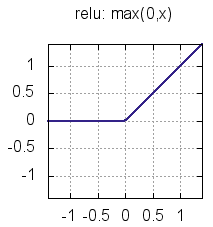
\includegraphics[scale=0.7]{img/act_relu.png}
   		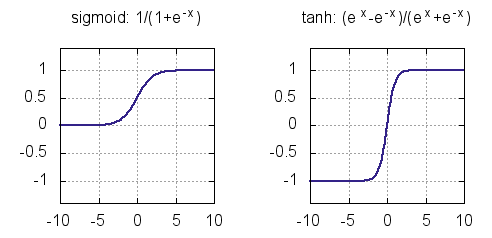
\includegraphics[scale=0.7]{img/act_sigm_tanh.png}
   		\caption{возможные функции активации}
   		\label{fig:act_functs}
    \end{figure}
\end{center}

Таким образом работа нейрона может быть представлена формулой:

{\large $$a^{l}_j = \sigma\left( \sum_k w^{l}_{jk} a^{l-1}_k + b^l_j \right)$$}

Где $a^l_j $ - выход нейрона $j$ слоя $l$, $ \sigma $ - функция активации, $w^l_{jk}$ - связи нейрона $j$ слоя $l$ c нейроном $k$ слоя $l-1$, $b^l_j$ - смещение нейрона $j$ слоя $l$

С целью оптимизации вычислений в данной работе нейрон не выделан как класс по описанным с следующем подразделе причинам.

\subsection{Слой}
Под слоем можно понимать набор нейронов на одном уровне. Каждый нейрон текущего слоя свзан со всеми нейронами предыдущего слоя. Поэтому рассчёт значений слоя требует порядка n\_in*n\_out операций, где n\_in - количество нейронов предыдыщего слоя, n\_out - текущего слоя. Рассчёт может быть удобно представлен в виде матричных операций. 

{\large $$a^{l} = \sigma\left( w^{l} a^{l-1} + b^l \right)$$}

Где $a^{l}$ и $b^{l}$ - векторы, состоящие из элеметнтов $a^{l}_j$ и $b^l_j$ соотвественно; $w^l$ - матрица коэффициентов связей между нейронами слоя $l$ и $l-1$ размерности n\_in*n\_out; $\sigma$ - применение функции активации ко все элементам вектора.

С первого взгляда такое представление не изменило ассимптотику алгоритма, однако вычисления будут происходить быстрее по следующим причинам:
\begin{enumerate}
\item Современные процессоры подерживают векторыне операции и скорость их выполенния выше последовательности аналогичных скалярных операций
\item В рамках интерпретируемого языка программирования Python библиотеки типа theano позволяют предварительно скомпилировать и оптимизировать векторные вычисления, что очень хорошо сказывается на производительности
\item theno позволяет проводить векторные вычисления на GPU, что чаcто позволяет их ускорить в 10 раз и более по сравнению с CPU.

Слой представлен классом HidelLayer.
\end{enumerate}

\subsection{Нейронная сеть}
Нейронная сеть представляет из себя набор последовательных слоёв. Позже сюда встявлю рисунок с архитектурой сети.

Нейронная сеть представлена классом MLP.
\subsection{Метод обучения}
Для обучения сети ипользован алгоритм обратного распространения ошибки.
Для обучения используется постоянный коэффициент, который является параметром алгоритма и передаётся заранее в метод.

Обучение сети реализовано в методе fit\_SGD класса MLP.
\subsection{Генетический алгоритм}
Генетический алгоритм по сути является эврестическим алгоритмом перебора. В данном случае пространством поиска являются начальные веса и смещения сети, которые и представляют из себя генотип.

Генетический алгоритм представлен классом GA.

\newpage\section{Разработка алгоритмов}

\subsection{Слой}

\subsection{Алгоритм обратного распространения ошибки}
Даный алгоритм базируется на четырёх основных уравнениях.

\subsection{Генетический алгоритм}

\newpage\section{Кодирование программы}
Прототипирование методов с описанием параметров и назначения

\newpage\section{Тестирование}
\subsection{Проверка на контроль ошибок}
\subsection{Контроль выполения задачи}
Данный подход должен продемонстрировать точность, на уровне аналогичных работ (применения многослойного перцептрона для прогнозирования направления биржевых котировок).

\newpage\section*{Выводы}
\addcontentsline{toc}{section}{Выводы}

\newpage\section*{Список источников}
\addcontentsline{toc}{section}{Список источников}
Тут надо по ГОСТу оформлять, а не как у меня было в старом курсаче

Список из старого курсача:
\begin{enumerate}
\item Канер С.  и др. Тестирование  программного  обеспечения.  Фундаментальные  концепции  
менеджмента бизнес-приложений.:  Пер.  с англ.  —  К.:  Издательство  «ДиаСофт»,  2001.  —  544  с.  
\item Бейзер Б. Тестирование черного ящика. Технологии функционального тестирования программного обеспечения и систем.  —  СПБ.: Питер, 2004.  —  318 с.: ил.
\par Интернет-источники:
\item http://www.intuit.ru/studies/courses/48/48/info
\item http://www.protesting.ru/testing/
\end{enumerate}


\newpage\section*{Приложения}
\addcontentsline{toc}{section}{Приложения}


\end{document}